
\section{Experimental results}
\label{sec:experimental-results}


% \end{table}
% In this section, we present a set of SystemJ benchmark programs in which
% real-time requirements should be met.  We have carried out a set of
% experiments to obtain BCRT and WCRT of the benchmark programs on two
% execution platforms called Java Optimized Processor(JOP)
% \cite{jop:jnl:jsa2007} and TP-JOP \cite{6119095}. JOP is a hardware
% implementation of the JVM which enables real-time execution of Java
% programs by translating Java bytecodes into a sequence of JOP's native
% instructions called \emph{microcode} which is time-predictable. As
% SystemJ's default compilation target is Java source code, JOP is an
% excellent platform which enables us to analyze timing properties of
% SystemJ program. On the other hand, there is also an option where
% compiled code could be more tightly coupled to specific platforms such
% as TP-JOP, which execute SystemJ's kernel statements more
% efficiently. By utilizing our internal tools in conjunction with
% Worst-Case-Execution-Time (WCET) analyzer \cite{jop:jnl:jsa2007}
% provided by JOP tools, we were able to estimate BCRT and WCRT of our
% benchmark programs: (full-name?) HRTCS, Stepper motor controller (Motor)
% \cite{}, Robot and Access Environment Control System (AECS) \cite{}.

% % HRTCS, as already illustrated in Section \ref{sec:intr-motiv}, tests
% % for an ability of one's responsiveness by generating green lights
% % between the real-time range \emph{M - N}. For AECS \ref{} we have
% % replaced the external timer with our delay constructs. Stepper motor
% % controller is originally introduced in \cite{Bourke2009a} which
% % converted into SystemJ.

% As one can see in Table \ref{table:benchmark}, BCRT and WCRT of overall
% programs are smaller when they run on TP-JOP. For example, WCRT and BCRT
% of HRTCS are \(\times\)11.9 and \(\times\)3.4 smaller, respectively, for
% TP-JOP (0.0028, 0.0329 ms) compared to JOP (0.0334, 0.1120 ms). On the
% other hand, required logical delays \emph{d} are generally bigger on
% TP-JOP e.g. \(\times\)4.5 - \(\times\)5.9 and \(\times\)30.9 in Motor
% and Robot respectively. It is expected as their BCRT and WCRT
% differences are bigger on TP-JOP.  This also led to greater increase in
% minimum upper real-time bounds \emph{N} for TP-JOP in every example.  In
% AECS, there are two clock-domains using delay constructs that each has
% their own BCRT and WCRT. Again, individual BCRT and WCRT is smaller
% whereas \emph{d} is bigger on TP-JOP. One important property to note
% here, is that BCRT and WCRT of any clock-domains are invariant of
% \emph{d} as explained in Section \ref{sec:intr-real-time}. It is our
% fundamental assumption to find \emph{d} in our benchmark programs.
% =======


We have carried out a number of experiments on a set of applications
with real-time constraints. The characteristics of the benchmark set
including required real-time waits and program sizes are shown in
Table~\ref{fig:benchlist}.  {\renewcommand{\arraystretch}{0.9}
%\renewcommand{\texttt}[1] {\begin{lstlisting}[language=Java,morekeywords={delay}] #1 \end{lstlisting}}
\begin{table}[h!]
	\scriptsize
	\centering
	\caption{An overview of the benchmark programs}
	\label{fig:benchlist}
	\scalebox{0.9}{
		\begin{tabular}{llp{0.5cm}p{1cm}}
\toprule
\emph{Benchmark}       & \emph{Delay constructs used in each CD} & \emph{\# of CDs} & 
\emph{Lines of code}        
\\ \midrule
HRTCS                  & \texttt{wait\_inbetween(50.3..200.3 ms)} ($CD1$) & 2                  & 56
\\ \midrule
\multirow{5}{*}{Motor} & \texttt{wait\_exact(2.4 ms)}        & \multirow{5}{*}{1} & \multirow{5}{*}{116} \\ 
											 &
                                                                                         \texttt{wait\_exact(1.667
                                                                                           ms)}      &                    &                      \\ 
											 &
                                                                                    \texttt{wait\_exact(0.05
                                                                                           ms)}       &                    &                      \\ 
											 &
                                                                                    \texttt{wait\_exact(0.3
                                                                                           ms)}        &                    &                      \\ 
											 &
                                                                                         \texttt{wait\_exact(0.733
                                                                                           ms)}      &                    &
\\ \midrule
\multirow{3}{*}{Printer}
& \texttt{wait\_inbetween(2.7..10.6 ms)} ($CD1$)      & \multirow{3}{*}{2}        & \multirow{3}{*}{39} \\
& \texttt{wait\_inbetween(1.2..30.3 ms)} ($CD2$)		  &														&											\\
& \texttt{wait\_inbetween(5.6..100.2 ms)} ($CD2$)     &														&											
\\ \midrule
\multirow{3}{*}{AECS} & \texttt{wait\_atleast(10000 ms)} ($CD1$) 
& \multirow{3}{*}{2} & \multirow{3}{*}{267} \\
& \texttt{wait\_exact(10000 ms)} ($CD2$) & & \\
& \texttt{wait\_exact(10000 ms)} ($CD2$) & &
\\ \bottomrule
\end{tabular}
}
\end{table}
}
{\renewcommand{\arraystretch}{0.6}
\begin{table*}[t!]
\centering
	\caption{Actual delays obtained for wait constructs in the
benchmark programs based on their BCRT and WCRT}
\resizebox{17.5cm}{!}{
\begin{tabular}{ c c l l l l l l }
	\toprule
	\multicolumn{2}{c}{} & \emph{HRTCS} & \emph{Motor} & \emph{Printer/CD1} &
	\emph{Printer/CD2} & \emph{AECS/CD1} &	\emph{AECS/CD2} \\ 
	\midrule
	\multicolumn{2}{c}{\emph{BCRT}}	& 0.0334 ms	& 0.0425 ms & 0.0190 ms &
	0.0263 ms & 0.1784 ms & 0.1284 ms\\ 
	\cmidrule(r){1-8}
	\multicolumn{2}{c}{\emph{WCRT}} &0.112 ms & 0.1096 ms & 0.0647 ms
	& 0.0491 ms & 0.3476 ms & 0.2991 ms\\ 
	\cmidrule(r){1-8}

	\multirow{2}{*}{Delay 1} & M..N & 50.3-200.3 ms	& 2.4-6.2493 ms	  &
	2.7-10.6 ms & 1.2-30.3 ms & 10000-19484.3481 ms& 10000-23278.2752 ms \\
	\cmidrule(r){2-8}
	& d &1506-1788 & 57 & 143-163 & 46-617 & 56062 &77844\\ 
	\cmidrule(r){1-8}
	\multirow{2}{*}{Delay 2} & M..N & N/A & 1.668-4.3855 ms & N/A &
	5.6-100.2 ms & N/A &10000-23278.2752 ms\\ 
	\cmidrule(r){2-8}
	& d & N/A & 40 & N/A & 213-2041 & N/A &77844\\ 
	\cmidrule(r){1-8}
	\multirow{2}{*}{Delay 3} & M..N & N/A & 0.05-0.2193 ms & N/A & N/A & N/A
	&N/A\\ 
	\cmidrule(r){2-8}
	& d & N/A & 2 & N/A & N/A & N/A &N/A\\ 
	\cmidrule(r){1-8}
	\multirow{2}{*}{Delay 4} & M..N & N/A & 0.3-0.8771 ms & N/A & N/A & N/A
	&N/A\\ 
	\cmidrule(r){2-8}
	& d & N/A & 8 & N/A & N/A & N/A &N/A\\ 
	\cmidrule(r){1-8}
	\multirow{2}{*}{Delay 5} & M..N & N/A & 0.733-1.9735 ms & N/A & N/A & N/A
	&N/A\\ 
	\cmidrule(r){2-8}
	& d & N/A & 18 & N/A
	& N/A & N/A &N/A\\ \bottomrule
\end{tabular}
}
\label{fig:comparison}
\end{table*}
}

\hj{ HRTCS is the human response system described in
  Section~\ref{sec:motivating-example}. HRTCS consists of 2 CDs, but
  only one with real-time wait.}

\hj{ Motor is a stepper motor controller from~\cite{Bourke2009a}, used
for producing monochrome images on paper by correct application of
current to a print head (a row of resistors). In this example, duration
of the current applied is controlled by the feedback logic using
real-time waits, which are expressed using reactive constructs.} It is a
synchronous program with 5 exact wait statements. 

\hj{ Printer is an example from~\cite{Schneider:1999:CRT:555233}, which
models a printer and a spooler in timed CSP. Its operation can be
described as follows: as soon as the spooler receives a print job it
passes it to the printer through a channel where actual printing process
take place.} Each spooler and printer process is mapped to a separate
CD. Spooler CD sends a job to the Printer CD between 2.7 to 10.6 ms
after receiving it from the environment (e.g. a user). On the other
hand, Printer CD notifies the environment that it starts printing
between 1.2 to 30.3 ms once it receives the job from the Spooler CD.
Actual print job is started between 5.6 to 100.2 ms after the
notification. In this example, bounded wait ensures that both; channel
communication and print job should occur within the specified amount of
time. % This example along with HRTCS demonstrates the use of non exact
% wait statements.

AECS (Access and Environmental Control System) is an application that
controls an intelligent room environment described in~\cite{aecs_ispa}.
AECS has 2 CDs; first one has one wait statement while the other has two
wait statements. The system is designed to measure how long the entrance
door to the room is being opened or to detect unknown entries (i.e.
intruders). For instance, the system triggers an alarm 10 seconds after
detection of an intruder or generates a beep sound when an entrance door
is being opened for the same amount of time. In the original AECS, the
system needed to interact with two external timers through input/output
signals in order to wait for a specific amount of time (e.g.
\texttt{TimerTriggered} in Figure~\ref{delaycode:a}). When the timer
expires, it notifies the system through the input signal
\texttt{TimeOut}, which is polled using the \texttt{await} statement.
The program has been modified such that the wait constructs replace
these external timers and corresponding interface (I/O) signals as shown
in Figure~\ref{delaycode:b}. With the new wait constructs, these timers
are not necessary and real-time waits can be expressed directly in the
SystemJ code.

\begin{figure}[h!]
	\vspace{-10pt}
	\centering
  \begin{SubFloat}{\label{delaycode:a}Original program}
      \scriptsize
		\begin{lstlisting}[style=sysj,morekeywords={abort,await,emit,present,trap,pause,exit,suspend}]
emit TimerTriggered;
trap(T){
  abort(DoorOpened){
    await(TimeOut);
    exit(T); 
  }
}
\end{lstlisting}
  \end{SubFloat}
  \hspace{1cm}%
  \begin{SubFloat}{\label{delaycode:b}Program with wait constructs}
		\begin{lstlisting}[style=sysj,morekeywords={abort,await,emit,present,trap,pause,exit,wait_atleast,suspend}]
// No emit statement
trap(T){
  abort(DoorOpened){
    wait_atleast (10000 ms);
    exit(T);  
  }
}
\end{lstlisting}
	\end{SubFloat}
\caption{Replacing external timer with wait\_atleast construct}
\label{delaycode}
\end{figure}



%Robot is an industrial automation application that consists of two
%manufacturing belts and a robotic arm that splits goods according to
%their volumes. 


%All these examples are written in
%the SystemJ language. The requirement to have deterministic or
%non-deterministic delays varies between each benchmark.  These delay
%requirements are shown in Table~\ref{fig:comparison} (\texttt{M..N}).


% In this section, we present a set of SystemJ benchmark programs in which
% real-time requirements should be met. We have carried out a set of
% experiments to obtain BCRT and WCRT of the benchmark programs on the
% execution platform called Java Optimized Processor(JOP)
% \cite{jop:jnl:jsa2007}. JOP is a hardware implementation of the JVM
% written in VHDL which enables real-time execution of Java programs by
% translating Java bytecodes into a sequence of JOP's native instructions
% called \emph{microcode} which is time-predictable. As SystemJ's default
% compilation target is Java source code, JOP is an excellent platform
% which enables us to analyze timing properties of SystemJ program.

% On the other hand, there is also an option where compiled code could be more
% tightly coupled to specific platforms such as TP-JOP, which execute SystemJ's
% kernel statements more efficiently.

We use the TP-JOP platform to carry out all our experiments. We
statically estimate the WCRT and BCRT of these benchmark applications
using our real-time analysis framework described previously in
Section~\ref{sec:stat-analys-comp-1}. The \textit{Safety Critical Java}
(SCJ) specification we use for real-time analysis avoids garbage
collection (GC) and hence, GC overheads and unpredictability are
completely avoided.

% We disable the \textit{Garbage Collector} (GC) in all experiments to
% avoid unwanted side-effects such as lengthening clock-domain logical
% tick times.

Table~\ref{fig:comparison} shows the result of our algorithm applied to
each benchmark program. Note that we allowed the compiler to relax the
upper real-time bounds for \texttt{wait\-\_exact} and
\texttt{wait\-\_inbetween} when it failed to find a feasible solution.
However, a user can prohibit such behavior using compiler switch as
described in Section~\ref{sec:tool-chain-flow}.

As a first step, BCRT and WCRT were calculated for all examples. Given
the real-time \texttt{wait\-\_inbetween (M..N)} provided by programmers,
required logical delay \textit{d} was determined by applying
Algorithm~\ref{alg:1}. In HR\-TCS, real-time delay of the range
50.3..200.3 (ms) is only satisfied when \emph{d} is between 1506 and
1788 (as shown previously in Section~\ref{sec:find-logic-delay}). Delay
2.7..10.6 (ms) is satisfied in Printer/CD1 with \emph{d} of 143..163.
Similarly, Printer/CD2 satisfies real-time ranges of 1.2..30.3 (ms) and
5.6..100.2 (ms) when \emph{d} is 46..617 and 213..2041, respectively. It
is then the compiler's job to statically choose one of the values in
this range.

% The upper bound \texttt{N} needed to be relaxed for all examples other
% than HRTCS to obtain a feasible \texttt{d}. Therefore,
On the other hand, Algorithm \ref{alg:2} is applied to those examples
where relaxation was required to determine the minimum upper real-time
bound \emph{N} such that there exists a solution for \emph{D} in
Algorithm \ref{alg:1}. This algorithm gives a unique number for logical
tick delay \emph{d} such that \emph{d} = Min(\emph{$S_2$}) =
Max(\emph{$S_1$}). The compiler, therefore, will choose \emph{d} based
on the newly computed \emph{N} for the examples: Motor and AECS.

\subsection{Improving results}

The previous results show that for HRTCS and Printer the compiler was
able to find \textit{d} without relaxing upper bound of wait
statements. Figure~\ref{fig:graph1} shows the accuracy of our results by
comparing between the programmer specified upper bounds
(Table~\ref{fig:benchlist}) and the actual bounds obtained using our
techniques (Table~\ref{fig:comparison}).
% relaxation. % AECS/CD1 wait specification is not included in
% Figure~\ref{fig:graph1}, because although it requires relaxation, the
% wait specification (Table~\ref{fig:benchlist}) does not have an upper
% bound.

\definecolor{cc1}{cmyk}{0,0,0,0}
\definecolor{cc2}{cmyk}{0,0,0,0.2}
\definecolor{cc3}{cmyk}{0,0,0,0.5}
\definecolor{cc4}{cmyk}{0,0,0,0.8}
\definecolor{cc5}{cmyk}{0,0,0,1}

\begin{figure}[h!]
	\centering
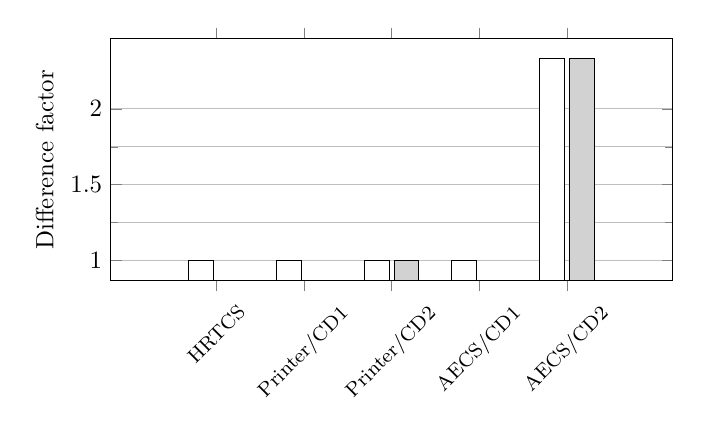
\begin{tikzpicture}[scale=0.9]
	\begin{axis}[
			ybar,xtick=data,
			symbolic x
			coords={HRTCS,Printer/CD1,Printer/CD2,AECS/CD1,AECS/CD2},
			height=5cm,
			width=9.5cm,
			minor y tick num=1,
			yminorgrids=true,
			ymajorgrids=true,
			ytick={0,0.5,...,2},
			enlarge x limits=0.3,
%      xlabel=Benchmark,
			x tick label style={rotate=45,font=\footnotesize},
			ylabel=Difference factor,
		]
			\addplot + [black,fill=cc1] coordinates
			{(HRTCS,1)(Printer/CD1,1)(Printer/CD2,1)(AECS/CD1,1)(AECS/CD2,2.33)};
			\addplot + [black,fill=cc2] coordinates 
                        {(Printer/CD2, 1)(AECS/CD2, 2.33)};
	\end{axis}
\end{tikzpicture}
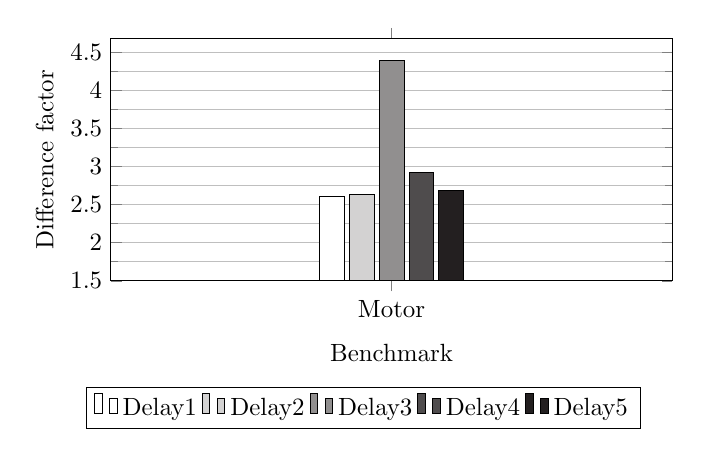
\begin{tikzpicture}[scale=0.9]
	\begin{axis}[
			ybar,xtick=data,
			symbolic x coords={Motor},
			ytick={0,0.5,...,5},
			ymin={1.5},
			minor y tick num=1,
			yminorgrids=true,
			ymajorgrids=true,
%      extra y ticks={2.5},
%      extra y tick labels={asdf},
%      extra y tick style={grid=major},
			height=5cm,
			width=9.5cm,
			xlabel=Benchmark,
			xlabel shift={4pt},
			ylabel=Difference factor,
			legend style={
				anchor=north,
				at={(0.45,-0.44)},
				legend columns=-1,
			}
%      nodes near coords
		]
			\addplot + [black,fill=cc1] coordinates
                        {(Motor, 2.60)};
			\addplot + [black,fill=cc2] coordinates
                        {(Motor, 2.63)};
			\addplot + [black,fill=cc3] coordinates
                        {(Motor, 4.39)};
			\addplot + [black,fill=cc4] coordinates
                        {(Motor, 2.92)};
			\addplot + [black,fill=cc5] coordinates
                        {(Motor, 2.69)};
			\legend{Delay1,Delay2,Delay3,Delay4,Delay5}
	\end{axis}
\end{tikzpicture}
\caption{Accuracy of the results}
\label{fig:graph1}
\end{figure}

There are two influential factors in determining the relaxation: 1)
execution speed of a target platform and 2) the nature of the program
that runs on this platform. Clock frequency of the processor directly
impacts the value of WCRT. On the other hand, programmer can write a
program such that large data (or control) computations in a single
logical tick increase WCRT of the program.  Assuming we do not change
the architecture of the execution platform (i.e. TP-JOP), the difference
factor can only be reduced by modifying the benchmark programs, as
stated earlier in Section~\ref{sec:extend-tehcn-vari}, such that the
critical paths are broken up using additional \texttt{pause} constructs,
thereby reducing the WCRT. Figure~\ref{fig:improv} shows segments of
code from AECS whose WCRT is reduced by such a technique.

\begin{figure}[h!]
	\centering
	\vspace{-10pt}
	\begin{SubFloat}{\label{fig:improv-a}Original program}
    \begin{minipage}[b]{0.45\linewidth}
		\begin{lstlisting}[style=sysj,morekeywords={present,emit,trap,pause,exit,delay,suspend}]
present(EntryRequest)
// obtaining 
// signal value
  id = #EntryRequest;
else
  id = #ExitRequest;
if(E.isValiedRequest(id)){
  // code ..
}
\end{lstlisting}
\end{minipage}
\end{SubFloat}
  \begin{SubFloat}{\label{fig:improv-b}Program with reduced WCRT}
    \centering
    \begin{minipage}[b]{0.45\linewidth}
		\begin{lstlisting}[style=sysj,morekeywords={emit,present,trap,pause,exit,delay,suspend}]
present(EntryRequest)
  id = #EntryRequest;
else
  id = #ExitRequest;
// Inserting pause
pause; 
if(E.isValiedRequest(id)){
  // code ..
}
\end{lstlisting}
		\end{minipage}
	\end{SubFloat}
	\caption{Improving WCRT by shortening a critical path}
	\label{fig:improv}
	\vspace{-10pt}
\end{figure}

In Figure~\ref{fig:improv-a}, the program simply checks for the id of a
person entering or exiting an intelligent room through the signals
called \texttt{EntryRequest} and \texttt{Exit\-Request}, and verifies
the id using data logic written in Java (\texttt{isValidRequest}). We
identified this as the critical execution path accounting for the WCRT.
In this case, we divide two consequtive statements, i.e.
\texttt{present} and \texttt{if}, by inserting \texttt{pause} such that
each of these statement is executed in two different ticks. The same
technique is applied to Motor example, which is purely
control-dominated, to reduce WCRT of the program. Note that we can also
optimize algorithms of the data computations used in each Java method to
reduce WCRT. However it is out of scope of this paper, hence not
discussed here.

The result of the upper bound relaxation with reduced WCRT is shown in
Figure~\ref{fig:graph2}.  The upper bounds for wait statements in
AECS/CD2 decreased by 11.81\%, while that for Motor example reduced from
6.42 to 8.05\%. This is expected since the amount of computation
required in control flow is less demanding than data and hence, breaking
the critical paths in Motor did not reduce WCRT as much as AECS/CD2.
Therefore, we can see from the result that the size of the relaxation
depends on how designers write their program as well as type of the
application (i.e. data or control dominated).

%For AECS/CD2, the upper bound has been reduced
%by 11.81\%, whereas for Motor, the reduced size ranges from 7.54 to
%8.05\% for each delay statement.  

\begin{figure}[ht!]
	\centering
%\begin{tikzpicture}[scale=0.9]
%  \begin{axis}[
%      ybar,xtick=data,
%      symbolic x
%      coords={AECS/CD2},
%      height=5cm,
%      width=9.5cm,
%      minor y tick num=1,
%      yminorgrids=true,
%      ymajorgrids=true,
%      xlabel=Benchmark,
%      ylabel=Percentage reduction,
%    ]
%      \addplot coordinates
%      {(AECS/CD2, 11.82)};
%  \end{axis}
%\end{tikzpicture}
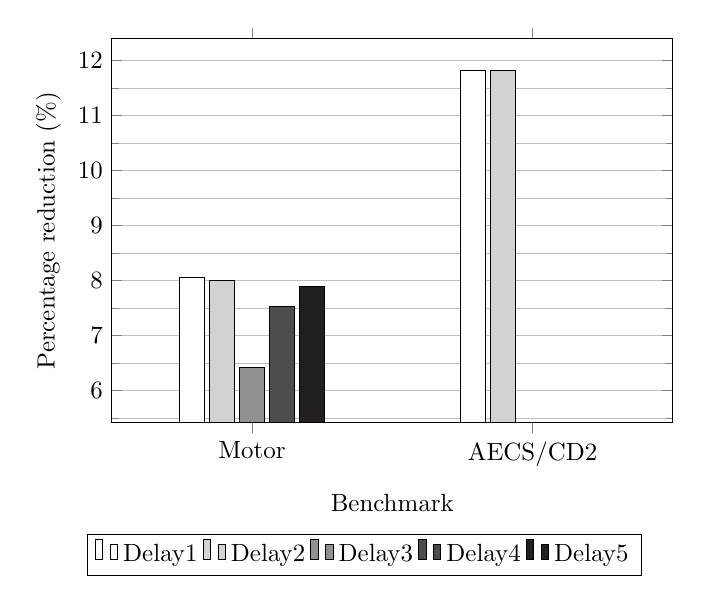
\begin{tikzpicture}[scale=0.9]
	\begin{axis}[
			ybar,xtick=data,
			symbolic x coords={Motor,AECS/CD2},
			ytick={0,1,...,12},
			ymin={6},
			minor y tick num=1,
			enlarge x limits=0.5,
			enlarge y limits=0.1,
			yminorgrids=true,
			ymajorgrids=true,
			height=7cm,
			width=9.5cm,
			xlabel=Benchmark,
			xlabel shift={4pt},
			ylabel=Percentage reduction (\%),
			legend style={
				anchor=north,
				at={(0.45,-0.29)},
				legend columns=-1,
			}
		]
			\addplot + [black,fill=cc1] coordinates
                        {(Motor, 8.05) (AECS/CD2, 11.82)};
			\addplot + [black,fill=cc2] coordinates
                        {(Motor, 8.00) (AECS/CD2, 11.82)};
			\addplot + [black,fill=cc3] coordinates
                        {(Motor, 6.42)};
			\addplot + [black,fill=cc4] coordinates
                        {(Motor, 7.53)};
			\addplot + [black,fill=cc5] coordinates
                        {(Motor, 7.89)};
			\legend{Delay1,Delay2,Delay3,Delay4,Delay5}
	\end{axis}
\end{tikzpicture}
\caption{Reduction in upper bound relaxation with improved WCRT}
\label{fig:graph2}
\end{figure}


% HRTCS, as already illustrated in Section \ref{sec:intr-motiv}, tests for an
% ability of one's responsiveness by generating green lights between the
% real-time range \emph{M - N}. For AECS \ref{} we have replaced the external
% timer with our delay constructs. Stepper motor controller is originally
% introduced in \cite{Bourke2009a} which converted into SystemJ.

% As one can see in Figure \ref{fig:comparison}, BCRT and WCRT of overall programs
% are smaller when they run on TP-JOP. For example, WCRT and BCRT of HRTCS are
% \(\times\)11.9 and \(\times\)3.4 smaller, respectively, for TP-JOP (0.0028,
% 0.0329 ms) compared to JOP (0.0334, 0.1120 ms). On the other hand, required
% logical delays \emph{d} are generally bigger on TP-JOP e.g. \(\times\)4.5 -
% \(\times\)5.9 and \(\times\)30.9 in Motor and Robot respectively. It is expected
% as their BCRT and WCRT differences are bigger on TP-JOP.
% This also led to greater increase in minimum upper real-time bounds \emph{N} for
% TP-JOP in every example.
% In AECS, there are two clock-domains using delay constructs that each has their
% own BCRT and WCRT. Again, individual BCRT and WCRT is smaller whereas \emph{d}
% is bigger on TP-JOP. One important property to note here, is that BCRT and WCRT
% of any clock-domains are invariant of \emph{d} as explained in Section
% \ref{sec:intr-real-time}. It is our fundamental assumption to find \emph{d} in
% our benchmark programs.
% >>>>>>> 4bffc4b1a43388f5ebf6cc737b9d3b246ee77dc7




%%% Local Variables: 
%%% mode: latex
%%% TeX-master: "template"
%%% End: 
